%% LyX 2.0.6 created this file.  For more info, see http://www.lyx.org/.
%% Do not edit unless you really know what you are doing.
\documentclass[oneside,english]{amsart}
\usepackage[T1]{fontenc}
\usepackage[latin9]{inputenc}
\usepackage{verbatim}
\usepackage{listings}
\usepackage{refstyle}
\usepackage{float}
\usepackage{textcomp}
\usepackage{amsthm}
\usepackage{amstext}
\usepackage{amssymb}
\usepackage{graphicx}

\makeatletter

%%%%%%%%%%%%%%%%%%%%%%%%%%%%%% LyX specific LaTeX commands.

\AtBeginDocument{\providecommand\figref[1]{\ref{fig:#1}}}
\floatstyle{ruled}
\newfloat{algorithm}{tbp}{loa}
\providecommand{\algorithmname}{Algorithm}
\floatname{algorithm}{\protect\algorithmname}
\RS@ifundefined{subref}
  {\def\RSsubtxt{section~}\newref{sub}{name = \RSsubtxt}}
  {}
\RS@ifundefined{thmref}
  {\def\RSthmtxt{theorem~}\newref{thm}{name = \RSthmtxt}}
  {}
\RS@ifundefined{lemref}
  {\def\RSlemtxt{lemma~}\newref{lem}{name = \RSlemtxt}}
  {}


%%%%%%%%%%%%%%%%%%%%%%%%%%%%%% Textclass specific LaTeX commands.
\numberwithin{equation}{section}
\numberwithin{figure}{section}
\newenvironment{lyxcode}
{\par\begin{list}{}{
\setlength{\rightmargin}{\leftmargin}
\setlength{\listparindent}{0pt}% needed for AMS classes
\raggedright
\setlength{\itemsep}{0pt}
\setlength{\parsep}{0pt}
\normalfont\ttfamily}%
 \item[]}
{\end{list}}
\theoremstyle{plain}
\newtheorem{thm}{\protect\theoremname}
  \theoremstyle{definition}
  \newtheorem{defn}[thm]{\protect\definitionname}
  \theoremstyle{definition}
  \newtheorem{example}[thm]{\protect\examplename}

%%%%%%%%%%%%%%%%%%%%%%%%%%%%%% User specified LaTeX commands.
\usepackage{algorithm}
\usepackage[noend]{algpseudocode}
\frenchspacing

\makeatother

\usepackage{babel}
  \providecommand{\definitionname}{Definition}
  \providecommand{\examplename}{Example}
\providecommand{\theoremname}{Theorem}

\begin{document}

\title{Efficient regexp implementation for finding parse trees}
\begin{abstract}
Regular expressions naturally and intuitively define ASTs that describe
the text that they're parsing. We describe a technique for building
up the complete parse tree resulting from matching a text against
a regular expression.

In standard TDFA matching, all paths through the NFA are walked simultaneously,
as if in different threads, where inside each thread, it is fully
known when which capture group was entered or left. We extend this
model to keep track of not just the last opening and closing of capture
groups, but all of them. We do this by storing, in every thread, using
the fly-weight pattern, a history of the all groups. Thus, we log
enough information during parsing to build up the complete AST at
the end of parsing.
\end{abstract}
\maketitle

\section{Introduction}

\global\long\def\regex{\text{\text{regular expression}}}
A regular expression can easily describe that a text matches a comma
separated values file, but it is unable to extract all the values.
Instead it will only give a single instance of values: \texttt{(({[}a-zA-Z
{]}+),(\textbackslash{}d+);)+} might describe a dataset of ASCII names
with their numeric label. Matching the regular expression on \texttt{``Tom
Lehrer,1;Alan Turing,2;''} will confirm that the list is well formed,
but the match will only contain \texttt{``Tom Lehrer''} for the
second capture group and \texttt{``1''} for the third. That is,
the full parse tree is: 

The amortized run time of our approach is $O(m\: n)$, where $m$
is the length of the regular expression and $n$ is the length of
the parsed string. This is asymptotically as fast as the best matchers
that don't extract parse trees. 


\subsection{Motivation}

This is the age of big data, and the first step of processing big
data is often to parse strings. As an example, consider log files..
What makes data huge is typically repetition. As Jacobs\cite{Jacobs2009}
noted, ``What makes most big data big is repeated observations over
time and/ or space,'' and thus log files grow large frequently. At
the same time, they provide important insight into the process that
they are logging, so their parsing and understanding is important. 

Regular expressions make for scalable and efficient lightweight parsers.\cite{Karttunen1996} 

Regular expression's parsing abilities have evoked Meiners to declare
that for intrusion detection, ``fast and scalable RE matching is
now a core network security issue.'' \cite{Meiners2010}

For example, Arasu et al.\cite{Arasu2012} demonstrate how regular
expressions are used in Bing to validate data, by checking whether
the names of digital cameras in their database are valid.

Parsers that can return abstract syntax trees are more useful than
ones that only give a flat list of matches. Of course only regular
grammars can be matched by our approach.

Let us recall what NFAs and DFAs are. A DFA is a state machine that
will walk over the transition graph, one step for every input
character. The choice of transition is limited by the transition's
character range. A transition can only be followed if the current
input character is inside transition's character range. NFAs differ
from DFAs in that for some input character and some state, there may
be more than applicable transition. If there is, an NFA will magically
guess the correct one. \figref{example-automaton} shows an example of
an NFA's transition graph. For the moment, let us discuss regular
expression matching on NFAs. Assuming that the NFA just magicly knows
the right transition lets us focus on the important things, greediness control
and capture groups.

\section{Algorithm}

Conceptually, our approach is the following pipeline of four stages.
\begin{enumerate}
  \item Parse the regular expression string into an AST.
  \item Transform the AST to an NFA.
  \item Transform the NFA to a DFA.
  \item Compactify the DFA.
\end{enumerate}

In reality, things are a little more involved, since the
transformation to DFA is lazy, and the compactification only happens
after no lazy compilation occurred in a while. Worse, compactification
can be undone if needed. We'll get back to these details in TODO
LATER. Let's discuss the stages in turn, starting with 2, since
parsing the regex grammar is reasonably straightforward.

\subsection{Thompson's construction} 

In step 2, we transform the AST of the regular expression into an NFA,
in a modified version of Thompson's NFA construction. TODO: ref. To
control greedines, or discern capture groups, our approach adds
$\epsilon$ transitions to the transition graph. An
$\epsilon$-transition has no input range assigned, and can thus always
be used. It does not consume an input character. The additions are
needed for greediness control and capture groups. Let's look at both,
in turn.

When the regular expression \texttt{(({[}a-zA-Z{]}+),(\textbackslash{}d+);)+} 
 is matched against input \texttt{bb},
capture group 2 is expected to match ``bb'', not ``b'', because
the matching of b+ is greedy. In the NFA, we model this by connecting
b+ to its following state via an $\epsilon$-transitions of \emph{low
priority}, SEE EXAMPLE. More generally, the NFA will prefer to follow
normal edges over those of low priority. Rather than formalize this
notion of preference, we come back to priorized edges when discussing
the transformation from NFA states to DFA states.

To model capture groups in the NFA, we add \emph{commit tags} to the
transition graph. The transition into a capture group is tagged by a
commit, the transition to leave a capture group is tagged by a another
commit. We distinguish opening and closing commits. The NFA keeps a
history for every transition with a commit. Each time the transition
is walked, the current position is added to its history. It is easy to
see that the entire match tree can be reconstructed from the list of
histories.

\begin{figure}
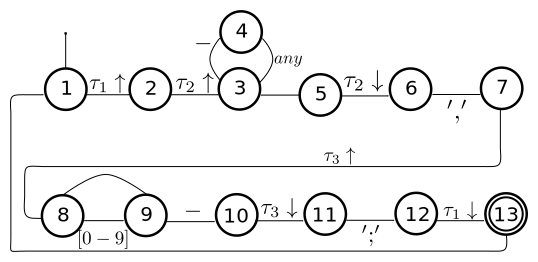
\includegraphics[width=0.69\textwidth]{graphs/lehrer_automaton}

\caption{\label{fig:example-automaton}
Automaton for \texttt{(({[}a-zA-Z{]}+),(\textbackslash{}d+);)+} }
\end{figure}

\subsection{DFAs}

Our above definition of regular expression assumes a machine that
guesses the correct transition through magic. To implement regular
expression matching without supernatural intervention, we lazily transform
the NFA to a DFA. 

A useful metaphor for regular expression matching is that of threads
\cite{Cox2007}. Whenever we aren't sure which transition to take,
we ``fork'' a thread for every option that we have. This way, when
the input is over, there must be at least one thread that guessed
correctly at all times. We use the word ``thread'' here to guide
intuition only. Our approach is not parallel. 

The key insight is that we keep all ``threads'' in lock-step. To
achieve this, we must be very specific about what constitutes the
state of a thread. Since every thread effectively simulates a different
NFA, the state inside of a thread contains exactly two items: the
NFA state it simulates, and the history for every tag. Now, the following
would be correct, although slow, implementation of a non-magic NFA
interpreter: whenever an input character is read, we can iterate over
all threads, kill the ones that have no legal transition for the input
character, and fork more threads as needed.

Trouble starts when we want to fork a thread for an NFA state that
is already running. Not is an explosion of threads bad for performance,
it would also lead to ambiguity: if the two threads disagree on the
histories, which one is correct?

The following algorithm takes as an input a set of threads, an NFA
transition graph, and an input character, and returns the set of threads
running after the input character has been read. It makes sure that
if there could be two threads with the same NFA state, the one that
follows greedy matching will survive.


\section{The TDFA powerset construction algorithm\label{sec:The-TNFA-algorithm}}

\global\long\def\naturals{\mathbb{N}}
\global\long\def\integers{\mathbb{Z}}
\global\long\def\pos{\mathbf{\mathbf{p}}}
Our algorithm is a modification of Laurikari's algorithm \cite{laurikari2000nfas},
which is itself a modified powerset construction algorithm \cite[p. 55]{Sipser2005}.
However instead of compiling the TNFA to a TDFA before matching, we
create the TDFA lazily as we match the string. For clarity, and because
the original description contains a few errors, we outline his algorithm
here, omitting his proof for correctness and termination.%
\begin{comment}
 In the TNFA algorithm, the state of the machine is not only determined
by the position in the state graph, but also by a number of positions
in the string that is read, that can later be used to construct the
subgroups of the match. 
\end{comment}
{} Our description adapts the thread metaphor of \cite{Cox2007}, where
each (T)NFA state describes the state of a single thread in a virtual
machine and the (T)DFA state is a collection of such threads.

Our algorithm runs two phases for each character read. First it creates
a new TDFA state from the current state and tries to map this state
and the instructions on the transition to a known state(as in \cite{laurikari2000nfas}),
then it executes the instructions found.

The memory model differs from other regular expression engines in
that locations are not stored in a fixed number of cells. Instead
each cell is the head of a singly linked list that describes the history
of the value. This allows us to extract all capture groups matching
a subpattern after the matching phase ended. Whenever threads are
forked, the histories of the matches sofar are shared, but we ensure
that further modifications will be thread-bound.

We need the following instructions:
\begin{description}
\item [{$n\leftarrow\mathbf{p}$}] Stores the current position in the input
string into the head of memory location $n$.
\item [{$n\leftarrow\pos+1$}] Stores the position after the current one
in the input string into the head of memory location $n$.
\item [{$n\leftarrow m$}] Replaces memory location $m$ with a copy of
head and history of memory location $n$.
\item [{$c\uparrow(n)$,}] $c\downarrow(n)$ Puts the current state of
memory location $n$ into the tail of the same memory location. The
two instructions don't differ in their effect, but in the order in
which they are executed.
\end{description}
\begin{algorithm}
\begin{lyxcode}
Name:~$interpret(input)$

Input:~~$input$~is~a~sequence~of~characters

Output:~a~tree~of~matching~capture~groups~for~the~regex

1.~Compute~all~states~after~start

$start\leftarrow epsilonClosure(startState,\varepsilon)$~and~execute~its~instructions

Initialize~TDFA~with~$start$~as~start~state.

$Q\leftarrow start$

  2.~Consume~string

for~all~indices~$pos$~and~values~$a$~of~$input$
\begin{lyxcode}
Try~to~find~a~mappable~state~$Q'$~with~$instructions$~on~the~transition~in~TDFA

if~$Q'$~was~found
\begin{lyxcode}
execute~$instructions$

jump~back~to~start~of~for~loop.
\end{lyxcode}
else
\begin{lyxcode}
$Q',instructions\leftarrow epsilonClosure(Q,a)$
\end{lyxcode}

\end{lyxcode}
\end{lyxcode}
\caption{TDFA from TNFA}
\end{algorithm}

\begin{defn}
For $I\subset\naturals$ and $n\in\naturals$, DFA state$\{(q_{i},(a_{ij})_{j=1..n}):i\in I\}$
is \emph{mappable} to another DFA state $\{(q_{i},(b_{ij})_{j=1..n}):i\in I\}$
iff there is a bijection $\nu$ such that $\forall i\in I,\, j=1..n:\,(a_{ij})=(\nu(b_{ij}))$.
Bijection $\nu$ is called the \emph{mapping}.\\
For example, $\{(q_{0},[4,3]),\,(q_{1},[2,1]),\,(q_{3},[2,3])\}$
is mappable to $\{(q_{0},[0,-2]),\,(q_{1},[2,1]),\,(q_{3},[2,-2])\}$
using mapping $1\mapsto1,\,3\mapsto-2,\,4\mapsto0$.

Let us first consider the caase where $N$ has no $\epsilon$ arrows
and no tags. Then we can construct the new transition function $\delta'$
as follows:

\[
\delta'(R,a)=\bigcup_{r\in R}\delta(r,a)\mbox{.}
\]

Now we need to consider the $\epsilon$ arrows, some of which contain
tags. We use the following notation:

For any state $R$ of $M$ we define $E(R)=\bigcup_{(r,t)\in R}e(q,t)$
to be a set of pairs. The first elements of the pairs are the states
that can be reached from $R$ by going along only $\epsilon$-arrows,
including the members of $R$ themselves. The second element of each
pair denotes the memory locations of all tags for their corresponding
NFA state.

\begin{algorithm}
\begin{lstlisting}[mathescape,tabsize=2]
Input: Graph of transitions for an NFA,
	Input character $a$,
	Input position $pos$,
	a set of threads $Q = {(q, [h_{1},\dots,h_{n}])}$,
	where $q$ is an NFA and $[h_{1},\dots,h_{n}]$ is an array of histories.
Output: Set of threads $R$.

$R\leftarrow\{\}$
Initialize empty stack $low$
Initialize empty stack $high$

// 1. push follow states with old histories.
For any $a$-consuming transition $t$ from any NFA state $q$ to $q'$ such that $(q, H) \in Q$.
	if $t$ has low priority push $(q', H)$ to $low$, else to $high$.
end for

// 2. Follow $\varepsilon$-transitions
While $high$ and $low$ are not both empty
	pop $(q', [h_{1},\dots,h_{n}]$ from $high$ if possible, else from $low$
	if $(q', H) \in R$ for some $H$, continue while
	add $(q', [h_{1},\dots,h_{n}])$ to $R$
	for all transitions $t$ from $q'$ to $q''$
		if $(q'', H) \in R$ for some $H$, continue for loop.
		if $t$ is tagged with an open or close tag:
			Choose $i$ such that $h_{i}$ is the history of  $t$'s open tag.
			Make a new history $h'$.
			$h_{i} \rightarrow h'$ (*)
			if $t$ has a open tag:
				Let $newHistories$ be $[\dots,h_{i-1},h',h_{i+1},\dots]$
				$h' \leftarrow pos+1$ (*)
			else, $t$ has a close tag:
				Choose $i'$ such that $h_{i'}$ is the history of  $t$'s open tag
				Make a new history $h''$
				$h_{i'} \rightarrow h''$ (*)
				$h'' \leftarrow pos$ (*)
				Commit $h'$
				Commit $h''$
				Let $newHistories$ be $[\dots,h_{i-1},h', \dots, h'',h_{i'+1},\dots]$
			end if
		end if				
				
		// Push according to priority of transition:
		if $t$ has low priority, push $(q'', newHistories)$ to $low$, else to $high$
	end for
end while
\end{lstlisting}

\caption{Compute the follow-up state for DFA state $Q$}
\end{algorithm}


\[
\delta^{\star}(R,a)=\{q\in Q:q\in E(\delta(r,a))\text{ for some }r\in R\}
\]
\end{defn}
\begin{example}
Computing the next state from the DFA state $(1[2,5,3,4],2[6,5,3,4],3[2,0,3,1],4[2,0,3,1],5[2,0,3,1],6[2,0,3,4],7[2,0,3,4],8[2,5,3,4])$,
which is the state after reading a single ``b'' input, in figure
\ref{fig:example-automaton}: \end{example}
\begin{enumerate}
\item Since only $3$ has a $b$ transition and no tags are written in consuming
transitions, $high=(4[2,0,3,1])$ after the initializing for loop
\item The state $4[2,0,3,1]$ is taken from the stack and added to $R$,
which is now $\{4[2,0,3,1]\}$ 

\begin{enumerate}
\item The transition $4\rightarrow5$ might be analysed first, but is added
to $low$, because for greedy consumption in the $+$ operator, the
backward way is prefered. The memory is not changed here.
\item Then the transition $4\rightarrow3$ is analysed and $3$ is added
to $high$ without changes in the memory.
\end{enumerate}
\item Now the state $3[2,0,3,1]$ is taken from the stack and added to $R$,
but since it has no $\epsilon$ exits, no further steps are taken
from here
\item The state $4[2,0,3,1]$ leads to $5[2,0,3,1]$
\item The state $5[2,0,3,1]$ leads to $6[2,0,3,7]$, because $\tau$ is
closed here.
\item The state $6[2,0,3,7]$ leads to $7[2,0,3,7]$.
\item The state $7[2,0,3,7]$ leads to $8[2,8,3,7]$, closing the $\sigma$
tag. 
\item The state $8[2,8,3,7]$ leads to $1[2,8,3,7]$
\item The state $1[2,8,3,7]$ leads to $2[9,8,3,7]$, reopening $\sigma$.
\item The state $2[9,8,3,7]$ would lead to $3[9,8,10,7]$, it is however
not added to $R$, because there is a different $3$ state (namely
$3[4,1,5,3]$) in $R$
\item Now, a mapping is searched by comparing the new DFA state $(1[2,8,3,7],2[9,8,3,7],3[2,0,3,1],4[2,0,3,1],5[2,0,3,1],6[2,0,3,7],7[2,0,3,7],8[2,8,3,7])$
to any old states, in our case $(1[2,5,3,4],2[6,5,3,4],3[2,0,3,1],4[2,0,3,1],5[2,0,3,1],6[2,0,3,4],7[2,0,3,4],8[2,5,3,4])$. 

\begin{enumerate}
\item Now the first NFA state has the memory $[2,8,3,7]$ in the new state
and $[2,5,3,4]$ in the old state. This adds the following constraints:

\begin{enumerate}
\item Memory locations $2$ and $3$ is mapped to themselves
\item Memory location $8$ is mapped to $5$
\item Memory location $7$ is mapped to $4$
\end{enumerate}
\item The second NFA state has the memory $[9,8,3,7]$ and $[6,5,3,4]$
respectively.

\begin{enumerate}
\item Memory location $9$ is mapped to $6$
\item Memory location $8$ is mapped to $5$, which conforms to the given
constraint from earlier
\item Memory location $7$ is mapped to $4$
\end{enumerate}
\item The third, forth, and fifth NFA state has identical memory, which
introduces the constraints for $0$ and $1$
\item The sixth and seventh NFA state conforms to the mapping of $7$ to
$4$
\item The eighth NFA state conforms to the mapping of $8$ to $5$.
\item This means that the new state is isomorphic to an existing state and
the mapping has been explicitly constructed. The newly introduced
locations are assigned the position of character read.
\end{enumerate}
\end{enumerate}

\section{TDFA with commits\label{sec:TNFA-with-hierarchical}}

The overall idea is simple: whenever the TDFA is reading in a run
of characters that belong to a capture group, we push the previous
one into our history and the work on current one. To implement this,
we introduce ``commits'' into the TDFA. On the level on the TNFA
the commits correspond to tags at the end of capture groups. Since
capture groups are nested, they form a tree. We will call this three
the match tree and will prove that we can reconstruct it. In it, we
store all runs that this capture group matches. The subnodes of a
hierarchy nodes correspond to the submatches of its capture group.We
will shortly discuss how to construct a TDFA that includes instructions
that \emph{commit} submatches into the hierarchy nodes.. Once we have
the instructions, during interpretation of the TDFA, whenever we encounter
an input character that closes a capture group, the TDFA will \emph{commit}
that capture group. To commit a substring into a hierarchy node has
the following semantics.

A hierarchy node, as a tree node, has a corresponding subtree. The
data in this subtree represents precisely the subtree of the AST that
is currently being matched. Upon commit of the hierarchy node, it
constructs this AST subtree, and stores it as a previous match. Iteratively,
this produces all matches of all capture groups.

\begin{figure}
\includegraphics[width=0.8\textwidth]{graphs/lehrer_match}

\includegraphics[width=0.8\textwidth]{graphs/lehrer_after}

\caption{Matching \texttt{(\textbackslash{}w+) (\textbackslash{}w+)}}


\end{figure}


\begin{comment}
if the current set of characters compare the current reading with
the previously longest read, keeping the longer one. n order to get
some more control over the overwriting of the tags, a separate \texttt{commit}
step can be introduced. Each nesting then would need a separate copy
of the temporary ``best'' match for a given group. For example \texttt{(((a+)b)+c)+}
would need two additional copies of the innermost group, to handle
conflicts. 

The intuition is to notice that two tags -- the opening and the corresponding
end tag -- always appear in order and the inner groups should not
spill over the end of the outer group. After each closing tag then
a commit is made, which handles whether the new or the old match is
longer. 
\end{comment}

\begin{example}
\begin{figure}
\begin{centering}
\includegraphics[width=0.75\textwidth]{graphs/abc}
\par\end{centering}

\caption{NFA about to be transformed.}
\end{figure}
In the following, the regex \texttt{(((a+)b)+c)+} will be converted
to a \textsc{dfa} lazily while matching the string ``abaababc'',
the resulting DFA can be seen in \ref{fig:lazy-dfa}:\end{example}
\begin{enumerate}
\item The starting state is $(1[-1,-2],2[0,-2])$ and the memory location
$0$ is initialized to hold the index $0$.
\item Now the letter a is read:

\begin{enumerate}
\item $2[0,-2]$ leads to $3[0,-2]$
\item $3[0,-2]$ leads to $2[0,-2]$
\item $3[0,-2]$ leads to $4[0,-2]$
\item $4[0,-2]$ leads to $5[0,1]$, with the instruction to write the index
to $1$ and commit the memory locations $(0,1)$ on level $3$ afterwards.
The hierarchical memory is now $c_{1}=nil,c_{2}=nil,c_{3}=(0,1)$,
where $(0,1)$ are the indeces, not the memory locations.
\end{enumerate}
\item Next the letter b is read:

\begin{enumerate}
\item $5[0,1]$ leads to $6[0,1]$
\item $6[0,1]$ leads to $1[0,1]$
\item $1[0,1]$ leads to $2[2,1]$, with the instruction to write the current
index to $2$.
\item $6[0,1]$ leads to $7[0,1]$
\item 7{[}0,1{]} leads to $8[0,1]$, with the instruction to commit to the
second level. The hierarchical memory is now $c_{1}=nil,c_{2}=(0,1),c_{3}=(0,1)$.
\end{enumerate}
\item Next the letter a is read:

\begin{enumerate}
\item $2[2,1]$ leads to $3[2,1]$
\item $3[2,1]$ leads to $2[2,1]$
\item $3[2,1]$ leads to $4[2,1]$
\item $4[2,1]$ leads to $5[2,3]$, with the instruction to write the current
index to memory location $3$ and commit the third level: $c_{1}=nil,c_{2}=(0,1),c_{3}=(2,3)$
\item We find, that this state is mappable to the previous state $(2[0,-2],3[0,-2],4[0,-2],5[0,1])$
with the mapping $2\rightarrow0,1\rightarrow-2$.
\end{enumerate}
\item Next the letter a is read:

\begin{enumerate}
\item $2[0,-2]$ leads to $3[0,-2]$
\item $3[0,-2]$ leads to $2[0,-2]$
\item $3[0,-2]$ leads to $4[0,-2]$
\item $4[0,-2]$ leads to $5[0,1]$, with the instruction to write the current
index to memory location $1$ and commit the third level: $c_{1}=nil,c_{2}=(0,1),c_{3}=(2,4)$.
\end{enumerate}
\item Next the letter b is read, but the transition is already known:

\begin{enumerate}
\item We write the current index into memory location $2$ and commit the
second level. Now the match $(2,4)$ is compared against the previous
match $(0,1)$, but the length of the new match is bigger, therefore
the new match overwrites the old one. $c_{1}=nil,c_{2}=(2,4),c_{3}=(2,4)$.
\end{enumerate}
\item Next the letter a is read, but the transition is already known:

\begin{enumerate}
\item We write the current index into memory location $-2$ (because of
the mapping) and commit $(2,-2)$ to the third level. $c_{1}=nil,c_{2}=(2,4),c_{3}=(5,6)$.
\end{enumerate}
\item Next the letter b is read, but the transition is already known:

\begin{enumerate}
\item We write the current index into memory location $2$ and commit to
the second level. The match $(5,6)$ is compared against the previous
match $(2,4)$, but the length of the old match is bigger, therefore
the old match is kept. $c_{1}=nil,c_{2}=(2,4),c_{3}=(5,6)$.
\end{enumerate}
\item Next the letter c is read:

\begin{enumerate}
\item $8[0,1]$ leads to $9[0,1]$
\item $9[0,1]$ leads to $1[0,1]$
\item $1[0,1]$ leads to $2[2,1]$, with the instruction to write the current
index to memory location $2$.
\item $9[0,1]$ leads to $10[0,1]$)
\item $10[0,1]$ leads to $11[0,1]$, with the instruction to commit to
the first level. $c_{1}=(2,4),c_{2}=(2,4),c_{3}=(5,6)$.
\end{enumerate}
\item Finally the end of the string is read.

\begin{enumerate}
\item We are in a finishing state $11[0,1]$, therefore the match succeeds.
The current commit of the top layer is returned: $c_{1}=(2,4)$.
\end{enumerate}
\end{enumerate}
\begin{figure}
\includegraphics[width=0.75\textwidth]{graphs/abc-dfa}

\caption{\label{fig:lazy-dfa}The DFA of \texttt{(?:(?:(a+)b)+c)+} matching
``abaababc''}


\end{figure}
\begin{comment}
This technique allows for programmers to extract parts of text with
great performance and flexibility regarding the extracted match. One
could imagine, that a programmer needs to extract a ideally complete
sample of formated text with optional parameters. Here, \texttt{\textsc{posix}}
regex would fail to deliver the best match in most cases. Such cases
can occur in data mining, in bioinformatics, both of which are handling
massive data, so that efficiency can be a problem.
\end{comment}



\section{Benchmark}


\section{Related work}

While there is no shortage of books discussing the usage of regular
expressions, the implementation side of regular expression has not
been so lucky. Cox is spot-on when he argues that innovations have
repeatedly been ignored and later reinvented \cite{Cox2007}. 

This paper is no exception. The authors of this paper had set out
to implement Laurikari's TDFA algorithm \cite{laurikari2000nfas},
only to discover that Laurikari's description of a TDFA is so far
from complete that it can rightfully only be called the sketch for
an algorithm. Only late in the process did we discover that the blanks
had already been filled by Kuklewicz in the course of his implementation
of TDFAs in Haskell \cite{Kuklewicz2007}. Kuklewicz enshrined his
added insight into Haskell library, but never published the algorithm
as a whole. If the history of regular expressions is evidence of one
thing, it is that source code is a terrible medium to convey algorithms. 

The situation dramatically improved with Cox's simple and concise
explanation of regular expression matching \cite{Cox2007}. It seems
ironic that this well-versed author published his influential work
on his website. Although the joke may be on Academia's side.

When the taciturn practioners acknowledge each other's work, we can't
help but disagree almost universally with the characterizations they
produce. Sulzmann and Lu \cite{sulzmann2012regular} call Kuklewicz's
work an ``implementation'' of Laurikari's algorithm, although Laurikari's
algorithm is far too incomplete for that statement to be fair. Laurikari's
algorithm is referred to as a POSIX-style automaton. In truth, Laurikari
leaves the matching strategy entirely open. It was Kuklewicz that
found out how to get POSIX-style matching out of Laurikari's TDFA. 

Cox says that Laurikari's TDFA is a reinvention Pike's published only
in code algorithm \cite{Pike1987}, which is Thompson's NFA with submatch
tracking. This seems unfair in that Laurikari's allows for far more
aggressive reusing of old states than what Thompson allows. This should
lead to Laurikari's TDFA having fewer states, and therefore better
performance, than even Google's RE2, which uses Pike's algorithm.
This is not confirmed by the benchmarks by Sulzmann and Lu \cite{sulzmann2012regular},
but they offer an explanation: in their profiling, they see that all
Haskell implementations spend considerable time decoding the input
strings. In other words, the measured performance is more of an artifact
of the programming environment used. 

Another mistake that permeates the scarce literature is to call regular
expression matching linear. As Sedgewick points out correctly \cite{Sedgewick1990},
Thompson's NFA matching is of complexity $O(mn)$, where $m$ is the
size of the input NFA, and $n$ is the size of the input string. To
call this linear requires to assume $m$ to be fix, which we cannot
bring ourselves to justify. It may well be true that, at present,
$m$ tends to be small. But that is a natural consequence of the algorithms
not scaling very well with $m$. If they did, that would allow for
fast feature extracting from text. Therefore, in this paper, we consider
the state of the art algorithms to be quadratic, since both $m$ and
$n$ are part of the input to a regular expression matcher. We cannot
rule out that a linear algorithm exists, in fact, we hope for it.
To insist that regular expression matching is done in linear time
is to insist that the optimal algorithm has already been found; that
is probably not true.

Sulzmann and Lu add to the table a new matching strategy that yields
good practical performance, although the theoretical bounds are considerably
worse than the state of the art, at $O(n^{2}m)$ \cite{sulzmann2012regular}.

\bibliographystyle{plain}
\bibliography{biblio}



\section*{Notes: }

Pseudocode

Beispiel(e) '(?:(?:(a+)b)+c)+'

Algorithm:

Definition:
\end{document}
